\documentclass[a4paper,fleqn]{cas-sc}

\usepackage[numbers,sort&compress]{natbib}
\usepackage{amsmath,amssymb}
\usepackage{booktabs}
\usepackage{xspace}
\usepackage{float}
\usepackage{placeins}

\newcommand{\AMO}{\mathrm{AMO}}
\newcommand{\ALO}{\mathrm{ALO}}
\newcommand{\TO}{\textsc{to}\xspace}

\newtheorem{lemma}{Lemma}
\newtheorem{proposition}{Proposition}
\newdefinition{definition}{Definition}
\newproof{proof}{Proof}

% No ORCID yet: hide the empty "ORCID(s):" footnote line (delete this if you add orcid=...).
\RenewDocumentCommand\printorcid{}{}

\begin{document}
\let\WriteBookmarks\relax
\renewcommand{\topfraction}{0.95}
\renewcommand{\bottomfraction}{0.85}
\renewcommand{\textfraction}{0.05}
\renewcommand{\floatpagefraction}{0.85}

\shorttitle{Assignment 1: N-Queens via SAT Encodings}
\shortauthors{Nguyen Cong Phuc}

\title[mode=title]{Assignment 1: Solving the N-Queens Problem via SAT Encodings and Comparison with Exact Solvers}

\author[1]{Nguyen Cong Phuc}[style=chinese]
\fnmark[1]
\ead{24021598@vnu.edu.vn}

\affiliation[1]{organization={Faculty of Information Technology, VNU University of Engineering and Technology},
            addressline={144 Xuan Thuy, Cau Giay Ward},
            city={Hanoi},
            postcode={100000},
            country={Vietnam}}

\fntext[1]{Student ID 24021598. Report for Assignment~1 of the course \emph{Modern Issues in Computer Science}, Semester I, 2026--2027.}

\begin{abstract}
This report presents our work for Assignment~1 in the course \emph{Modern Issues in Computer Science}, focusing on modeling and solving the N-Queens problem using Boolean Satisfiability (SAT). We formulate the problem into Conjunctive Normal Form (CNF) with various At-Most-One (AMO) encoding techniques, including five self-implemented encodings (pairwise, sequential counter, binary, commander, and product) and six encodings from the PySAT library. We evaluate the generated CNF formulas using four SAT solvers (CaDiCaL, Glucose, Kissat, MiniSat) and compare their performance against exact solvers including Google OR-Tools CP-SAT, Gurobi MIP, and CPLEX under single-thread settings with a 60\,s timeout. The experimental results show that linear encodings scale significantly better than the naive pairwise encoding on large boards ($n=512$ and $n=1000$). We also examine the practical benefits of adding redundant column at-least-one clauses and verify all solution counts against the OEIS A000170 sequence up to $n=12$.
\end{abstract}

\begin{keywords}
N-Queens \sep SAT encoding \sep at-most-one constraint \sep CDCL \sep constraint programming \sep integer programming
\end{keywords}

\maketitle

\section{Introduction}\label{sec:intro}

The $n$-queens problem is a classic combinatorial problem where $n$ queens must be placed on an $n\times n$ chessboard such that no two queens attack each other across any row, column, or diagonal. In computer science, it provides an intuitive yet structured benchmark for studying constraint satisfaction and exact search methods.

In this assignment, we focus on translating the $n$-queens problem into propositional logic formulas in Conjunctive Normal Form (CNF). The main challenge lies in translating the At-Most-One (AMO) constraints on rows, columns, and diagonals into clauses efficiently. While naive pairwise encoding is simple, it generates $O(k^2)$ clauses per line, causing formula size to explode on large boards. To address this, several advanced encoding techniques with auxiliary variables have been proposed in the literature.

The main objectives of this assignment include:
\begin{itemize}
\item Implementing five AMO encodings from scratch (pairwise, sequential counter, binary, commander, product) under a common Python interface, and wrapping six PySAT cardinality encodings.
\item Verifying the correctness of the encodings through unit tests, independent board verification, and comparing solution counts with OEIS A000170 up to $n=12$.
\item Benchmarking the encodings across four modern SAT solvers (CaDiCaL, Glucose, Kissat, MiniSat) on boards up to $n=512$ and $n=1000$.
\item Evaluating the effect of adding redundant column at-least-one (ALO) clauses on solver runtimes.
\item Comparing SAT performance with exact solvers including Google OR-Tools CP-SAT, Gurobi MIP, and CPLEX under consistent single-thread settings.
\end{itemize}
All experimental numbers in this report are generated directly from the CSV logs in the project repository (Section~\ref{sec:data}).

The rest of this report is organized as follows: Section~\ref{sec:background} introduces the problem formulations; Section~\ref{sec:method} details the SAT encoding approach; Section~\ref{sec:experiments} presents the experimental setup and results; and Section~\ref{sec:conclusion} concludes the report.

\section{Background}\label{sec:background}

\subsection{Problem definition}

We index rows and columns from $0$ to $n-1$. Two queens at cells $(r,c)$ and $(r',c')$ attack each other if they share a row ($r=r'$), a column ($c=c'$), a main diagonal ($r-c=r'-c'$), or an anti-diagonal ($r+c=r'+c'$). Since each row must contain exactly one queen, a candidate solution can be represented as a vector $q=(q_0,\dots,q_{n-1})$ where $q_r$ is the column index of the queen in row $r$, satisfying for all $r\ne s$:
\begin{equation}\label{eq:perm}
q_r \neq q_s, \qquad q_r + r \neq q_s + s, \qquad q_r - r \neq q_s - s .
\end{equation}
The number of distinct valid placements $Q(n)$ corresponds to the OEIS sequence A000170~\citep{oeisA000170}: 1, 0, 0, 2, 10, 4, 40, 92, 352, 724, 2680 and 14\,200 for $n=1,\dots,12$.

We denote a \emph{line} as any set of squares where at most one queen may stand: the rows $R_r$, the columns $C_c$, the main diagonals $D^-_d=\{(r,c): r-c=d\}$, and the anti-diagonals $D^+_s=\{(r,c): r+c=s\}$. There are $2(2n-1)$ diagonal lines in total. The four single-cell corner lines cannot have conflicts and are ignored, leaving $2(2n-3)$ diagonal lines with at least two squares, denoted as $\mathcal{D}$.

\subsection{Integer and constraint programming formulations}

With a binary decision variable $x_{r,c} \in \{0, 1\}$ indicating whether a queen is placed on square $(r,c)$, the problem can be formulated as a 0-1 Integer Linear Program (ILP/MIP):
\begin{align}
\textstyle\sum_{c} x_{r,c} &= 1 && \forall r, \label{eq:ilp-row}\\
\textstyle\sum_{r} x_{r,c} &= 1 && \forall c, \label{eq:ilp-col}\\
\textstyle\sum_{(r,c)\in D} x_{r,c} &\le 1 && \forall D\in\mathcal{D}, \label{eq:ilp-diag}\\
x_{r,c} &\in\{0,1\} && \forall r,c. \label{eq:ilp-bin}
\end{align}
This formulation consists of $n^2$ binary variables and $6n-6$ linear constraints (for $n\ge2$). We evaluate this 0-1 model using Gurobi~\citep{gurobi2025}, CPLEX~\citep{cplex2022}, and OR-Tools CP-SAT~\citep{perron2026cpsat}.

Alternatively, the Constraint Programming (CP) formulation uses $n$ integer variables $q_r \in \{0,\dots,n-1\}$ and three global constraints:
\begin{equation}\label{eq:cp}
\textsc{AllDifferent}(q_r)_{r},\qquad \textsc{AllDifferent}(q_r+r)_{r},\qquad \textsc{AllDifferent}(q_r-r)_{r}.
\end{equation}
We evaluate this formulation using OR-Tools CP-SAT.

\subsection{SAT solving and AMO encodings}

A SAT problem asks whether a Boolean formula in Conjunctive Normal Form (CNF) is satisfiable. Modern SAT solvers use Conflict-Driven Clause Learning (CDCL)~\citep{marques1999grasp,een2003minisat}, combining unit propagation, decision heuristics, and conflict analysis to solve large instances efficiently. We use four solvers available through the PySAT library~\citep{ignatiev2018pysat}: MiniSat~2.2, Glucose~4.1, CaDiCaL~1.9.5, and Kissat~4.0.4.

Given a set of literals $X=\{x_1,\dots,x_k\}$, the At-Least-One constraint $\ALO(X)$ is represented by a single clause $(x_1\vee\dots\vee x_k)$. The At-Most-One constraint $\AMO(X)$ requires at most one literal in $X$ to be true. Several methods exist to encode AMO into CNF:
\begin{itemize}
\item \emph{Pairwise}: Adds a binary clause $(\neg x_i \lor \neg x_j)$ for every pair $i < j$. It requires no auxiliary variables but uses $\binom{k}{2} = O(k^2)$ clauses.
\item \emph{Sequential counter}~\citep{sinz2005towards}: Uses $k-1$ auxiliary variables to propagate partial sums, requiring $O(k)$ clauses.
\item \emph{Binary}~\citep{frisch2005solving}: Encodes the active literal index in $O(\log k)$ bits, requiring $O(k \log k)$ clauses.
\item \emph{Commander}~\citep{klieber2007efficient}: Groups literals into subsets with group leaders, recursively applying AMO in $O(k)$ clauses.
\item \emph{Product}~\citep{chen2010new}: Maps literals onto a 2D grid of size $\sqrt{k} \times \sqrt{k}$, reducing both clauses and auxiliary variables to $O(k)$ and $O(\sqrt{k})$.
\end{itemize}

\section{SAT-based approach}\label{sec:method}

\subsection{Variables and constraints}

For each cell, the Boolean variable $x_{r,c}$ states that a queen stands on $(r,c)$; in DIMACS numbering, $x_{r,c}$ is variable $rn+c+1$, so the board uses variables $1,\dots,n^2$. Given an AMO encoding $E$, which maps a set of literals to a set of clauses over those literals and fresh auxiliary variables, the formula is
\begin{equation}\label{eq:cnf}
F_n(E) \;=\; \bigwedge_{r} \big[\ALO(R_r)\wedge E(R_r)\big] \;\wedge\; \bigwedge_{c} \big[\ALO(C_c)\wedge E(C_c)\big] \;\wedge\; \bigwedge_{D\in\mathcal{D}} E(D),
\end{equation}
where each call to $E$ draws its auxiliary variables from a global counter so that no two lines share them. The column ALO clauses are redundant: exactly one queen per row places $n$ queens, and at most one queen in each of the $n$ columns then forces exactly one per column (pigeonhole principle). They are kept by default because redundant clauses may help propagation; Section~\ref{sec:ablation} measures their effect.

\subsection{AMO encodings implemented}\label{sec:encodings}

Let $X=(x_1,\dots,x_k)$ be the literals of one line.

\paragraph{Pairwise.} $\bigwedge_{1\le i<j\le k}(\neg x_i\vee\neg x_j)$.

\paragraph{Sequential counter~\citep{sinz2005towards}.} With auxiliary variables $s_1,\dots,s_{k-1}$, where $s_i$ means ``some of $x_1,\dots,x_i$ is true'':
\begin{equation}
(\neg x_1\vee s_1)\wedge\bigwedge_{i=2}^{k-1}\big[(\neg x_i\vee s_i)\wedge(\neg s_{i-1}\vee s_i)\wedge(\neg x_i\vee\neg s_{i-1})\big]\wedge(\neg x_k\vee\neg s_{k-1}).
\end{equation}

\paragraph{Binary~\citep{frisch2005solving}.} With $m=\lceil\log_2 k\rceil$ bits $b_1,\dots,b_m$, literal $x_i$ is given the code $i-1$ in binary; $\beta_{i,j}$ is $b_j$ if bit $j$ of $i-1$ is one and $\neg b_j$ otherwise:
\begin{equation}
\bigwedge_{i=1}^{k}\bigwedge_{j=1}^{m}(\neg x_i\vee \beta_{i,j}).
\end{equation}

\paragraph{Commander~\citep{klieber2007efficient}.} $X$ is split into groups $G_1,\dots,G_g$ of at most three literals. Each group with two or more literals receives a commander $c_j$ with $c_j\leftrightarrow\bigvee G_j$; a singleton group uses its own literal as commander. The encoding is
\begin{equation}
\bigwedge_{j}\Big[\mathrm{Pairwise}(G_j)\wedge\bigwedge_{x\in G_j}(\neg x\vee c_j)\wedge\big(\neg c_j\vee\textstyle\bigvee G_j\big)\Big]\;\wedge\;\mathrm{Commander}(c_1,\dots,c_g),
\end{equation}
applied recursively until at most three literals remain, which are then encoded pairwise.

\paragraph{Product~\citep{chen2010new}.} The literals are laid row by row on a $p\times q$ grid with $q=\lceil k/\lceil\sqrt{k}\rceil\rceil$ columns and $p=\lceil k/q\rceil$ rows. With row variables $u_1,\dots,u_p$ and column variables $v_1,\dots,v_q$, and $x_{a,b}$ the literal in cell $(a,b)$,
\begin{equation}
\bigwedge_{a,b}\big[(\neg x_{a,b}\vee u_a)\wedge(\neg x_{a,b}\vee v_b)\big]\;\wedge\;\mathrm{Product}(u_1,\dots,u_p)\wedge\mathrm{Product}(v_1,\dots,v_q),
\end{equation}
recursively, with the pairwise encoding for $k\le4$.

\paragraph{PySAT encodings.} \texttt{CardEnc.atmost} with bound one provides the pairwise, sequential counter (\texttt{seqcounter}), binary (\texttt{bitwise}), ladder, totalizer and cardinality network (\texttt{cardnetwrk}) encodings~\citep{ignatiev2018pysat}.

Table~\ref{tab:sizes} summarizes the theoretical size complexity of each encoding. While the naive pairwise encoding requires $\Theta(n^3)$ clauses across the chessboard lines, the sequential counter, commander, and product encodings achieve linear $\Theta(n^2)$ total clauses by introducing auxiliary variables.

\begin{table}[pos=!htb]
\caption{Size of one AMO constraint over $k$ literals (own implementations) and order of the whole $n$-queens formula.}\label{tab:sizes}
\centering
\begin{tabular}{@{}llll@{}}
\toprule
Encoding & Clauses & Auxiliary variables & Clauses in $F_n$ \\
\midrule
Pairwise   & $k(k-1)/2$ & $0$ & $\Theta(n^3)$ \\
Sequential & $3k-4$ & $k-1$ & $\Theta(n^2)$ \\
Binary     & $k\lceil\log_2 k\rceil$ & $\lceil\log_2 k\rceil$ & $\Theta(n^2\log n)$ \\
Commander (groups of 3) & $\approx 3.5k$ & $\approx k/2$ & $\Theta(n^2)$ \\
Product    & $2k+4\sqrt{k}+O(k^{1/4})$ & $2\sqrt{k}+O(k^{1/4})$ & $\Theta(n^2)$ \\
\bottomrule
\end{tabular}
\end{table}

\subsection{Implementation and verification}\label{sec:implementation}

The implementation is structured as a modular Python package. Every AMO encoder follows a unified signature \texttt{(lits, next\_var) -> (clauses, next\_var)}, allocating auxiliary variables incrementally from \texttt{next\_var} to avoid variable ID collisions across lines. The six PySAT encodings are wrapped under the same interface.

To enumerate all solutions, whenever a satisfying model is found, we add a blocking clause $\bigvee_r \neg x_{r,q_r}$ restricted strictly to the $n^2$ board variables. This prevents duplicate counting even when encodings allow multiple valid assignments to auxiliary variables.

Correctness was validated at three levels: (i) exhaustive truth-table verification of each encoding against the AMO definition for small $k$ and sampled tests for larger $k$; (ii) comparing the full solution sets against a naive permutation search for $n\le 7$; and (iii) verifying the enumerated solution counts against the OEIS A000170 sequence for $n\le 12$ (Section~\ref{sec:counting}).

\FloatBarrier
\section{Computational experiments}\label{sec:experiments}

\subsection{Experimental setup}

All experiments ran on an Intel Core i5-7267U CPU at 3.1\,GHz (two cores, four threads, 8\,GB RAM) under macOS~13.7.8, with Python~3.14.8, PySAT~1.9.dev15, OR-Tools~9.15, Gurobi~13.0.3, and CPLEX~22.1.2. Solvers were evaluated under single-thread execution with a 60\,s timeout per run. Each run was executed in a separate process. The time limit applies to the solver call only; building the CNF in Python is measured separately and limited to 900\,s. For each configuration, $n$ was increased until the first timeout, and larger boards were not attempted (shown as ``--''). The pairwise encodings were limited to $n\le128$ because their $\Theta(n^3)$ clauses exceed the 8\,GB of memory beyond that size. CPLEX CP Optimizer could not be evaluated because its \texttt{cpoptimizer} executable is not included in the pip package and was not installed.

Community editions of Gurobi and CPLEX enforce variable caps of 2000 and 1000 variables, allowing them to solve up to $n=44$ and $n=31$ respectively (denoted as ``lic.'' in tables). Five experiments were conducted: formula size, single-solution SAT solving ($n\le 512$), all-solution counting ($n\le 12$), column ALO ablation, and comparison with CP and MIP solvers.

\subsection{Correctness and enumeration of all solutions}\label{sec:counting}

Table~\ref{tab:count} reports the enumeration of all solutions for $n\le12$. For each of the 132 combinations of board size and encoding, the number of solutions enumerated by CaDiCaL with blocking clauses equals OEIS A000170, including the unsatisfiable cases $n=2$ and $n=3$, and every enumerated solution passed the independent check. Together with the semantic tests of Section~\ref{sec:implementation}, this gives strong evidence that the eleven encodings are correct.

In this setting the formulas are small and the cost is dominated by the number of solver calls (14\,200 at $n=12$). The pairwise encoding, which has no auxiliary variables, is the fastest SAT variant (2.40\,s at $n=12$) and the PySAT totalizer the slowest (5.84\,s). Enumeration through incremental SAT is about two to five times faster than the native enumeration of CP-SAT (11.0--11.9\,s), but a dedicated bitmask backtracking search remains faster still (0.45\,s, in pure Python), since it exploits the structure of the problem directly (Figure~\ref{fig:count}).

\begin{table}[pos=!htb]
\caption{Enumeration of all solutions. ``Correct encodings'': number of encodings whose enumerated count equals OEIS A000170. Times in seconds; the SAT columns give the fastest and slowest of the eleven encodings (CaDiCaL, blocking clauses).}\label{tab:count}
\centering\small
\begin{tabular}{@{}rrcrrrrr@{}}
\toprule
$n$ & solutions & correct encodings & backtracking & CP-SAT int & CP-SAT 0-1 & SAT fastest & SAT slowest \\
\midrule
1 & 1 & 11/11 & $<$0.01 & 0.04 & $<$0.01 & $<$0.01 & $<$0.01 \\
2 & 0 & 11/11 & $<$0.01 & 0.02 & $<$0.01 & $<$0.01 & $<$0.01 \\
3 & 0 & 11/11 & $<$0.01 & 0.02 & $<$0.01 & $<$0.01 & $<$0.01 \\
4 & 2 & 11/11 & $<$0.01 & 0.03 & $<$0.01 & $<$0.01 & $<$0.01 \\
5 & 10 & 11/11 & $<$0.01 & 0.03 & $<$0.01 & $<$0.01 & $<$0.01 \\
6 & 4 & 11/11 & $<$0.01 & 0.01 & $<$0.01 & $<$0.01 & $<$0.01 \\
7 & 40 & 11/11 & $<$0.01 & 0.01 & $<$0.01 & $<$0.01 & $<$0.01 \\
8 & 92 & 11/11 & $<$0.01 & 0.04 & 0.02 & $<$0.01 & 0.02 \\
9 & 352 & 11/11 & $<$0.01 & 0.10 & 0.11 & 0.04 & 0.09 \\
10 & 724 & 11/11 & 0.01 & 0.63 & 0.37 & 0.07 & 0.24 \\
11 & 2\,680 & 11/11 & 0.09 & 2.42 & 2.61 & 0.42 & 2.42 \\
12 & 14\,200 & 11/11 & 0.45 & 11.9 & 11.0 & 2.40 & 5.84 \\
\bottomrule
\end{tabular}

\end{table}

\begin{figure}[pos=!htb]
\centering
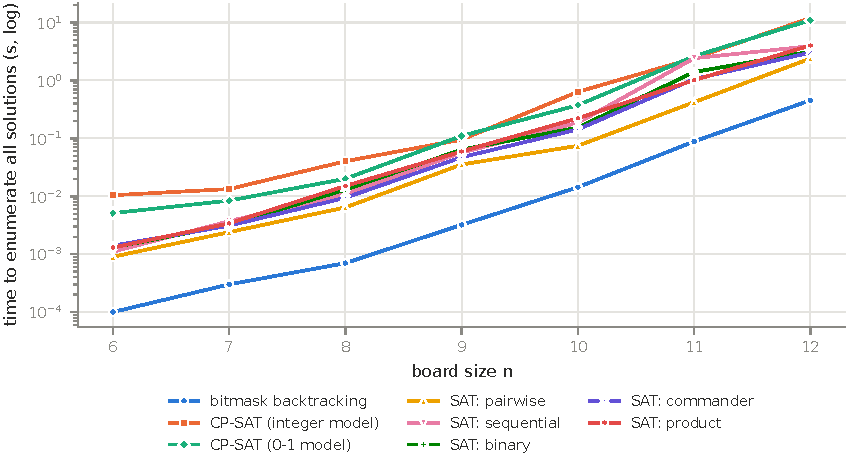
\includegraphics[width=0.9\textwidth]{figures/fig_count.pdf}
\caption{Time to enumerate all solutions ($6\le n\le 12$, log scale): bitmask backtracking, CP-SAT with both models, and incremental SAT with the five own encodings.}\label{fig:count}
\end{figure}

\subsection{Size of the encodings}

Table~\ref{tab:size} and Figure~\ref{fig:size} give the measured size of $F_n(E)$. The measurements agree with the analysis of Section~\ref{sec:encodings}. The two cubic encodings grow fastest: the pairwise formula already has 3.46 million clauses at $n=128$, and the PySAT totalizer reaches 29.8 million clauses at $n=256$. Among the other encodings, the product encoding produces the fewest clauses from $n=64$ on (2.44 million at $n=512$), followed by the sequential counter (3.13 million) and the commander encoding (3.65 million). The binary encoding introduces by far the fewest auxiliary variables (0.29 million at $n=512$).

\begin{table}[pos=!htb]
\caption{Number of variables and clauses of $F_n(E)$. Each own encoding is followed by its PySAT counterpart, if any; encodings available only in PySAT are below the rule. ``--'': not generated (memory cap for pairwise, build limit for the totalizer).}\label{tab:size}
\centering\small
\begin{tabular}{@{}lrrrrrrrr@{}}
\toprule
Encoding & \multicolumn{2}{c}{$n=8$} & \multicolumn{2}{c}{$n=64$} & \multicolumn{2}{c}{$n=256$} & \multicolumn{2}{c}{$n=512$} \\
\cmidrule(lr){2-3}\cmidrule(lr){4-5}\cmidrule(lr){6-7}\cmidrule(lr){8-9}
 & vars & clauses & vars & clauses & vars & clauses & vars & clauses \\
\midrule
pairwise & 64 & 744 & 4\,096 & 428\,864 & -- & -- & -- & -- \\
PySAT pairwise & 64 & 744 & 4\,096 & 428\,864 & -- & -- & -- & -- \\
sequential & 274 & 604 & 20\,098 & 47\,756 & 326\,146 & 780\,812 & 1\,307\,650 & 3\,134\,476 \\
PySAT seqcounter & 270 & 600 & 20\,094 & 47\,752 & 326\,142 & 780\,808 & 1\,307\,646 & 3\,134\,472 \\
binary & 174 & 728 & 6\,136 & 95\,576 & 76\,788 & 2\,053\,464 & 287\,730 & 9\,262\,424 \\
PySAT bitwise & 170 & 724 & 6\,132 & 95\,572 & 76\,784 & 2\,053\,460 & 287\,726 & 9\,262\,420 \\
commander & 146 & 618 & 11\,958 & 55\,022 & 195\,936 & 909\,198 & 784\,502 & 3\,652\,158 \\
product & 236 & 652 & 12\,476 & 45\,620 & 125\,800 & 631\,720 & 459\,472 & 2\,439\,384 \\
\midrule
PySAT ladder & 346 & 996 & 20\,842 & 65\,620 & 329\,194 & 1\,049\,044 & 1\,313\,770 & 4\,195\,284 \\
PySAT totalizer & 740 & 1\,458 & 96\,932 & 522\,074 & 2\,075\,300 & 29\,842\,842 & -- & -- \\
PySAT cardnetwrk & 872 & 1\,264 & 67\,960 & 96\,240 & 1\,107\,448 & 1\,564\,656 & 4\,443\,128 & 6\,275\,056 \\
\bottomrule
\end{tabular}

\end{table}

\begin{figure}[pos=!htb]
\centering
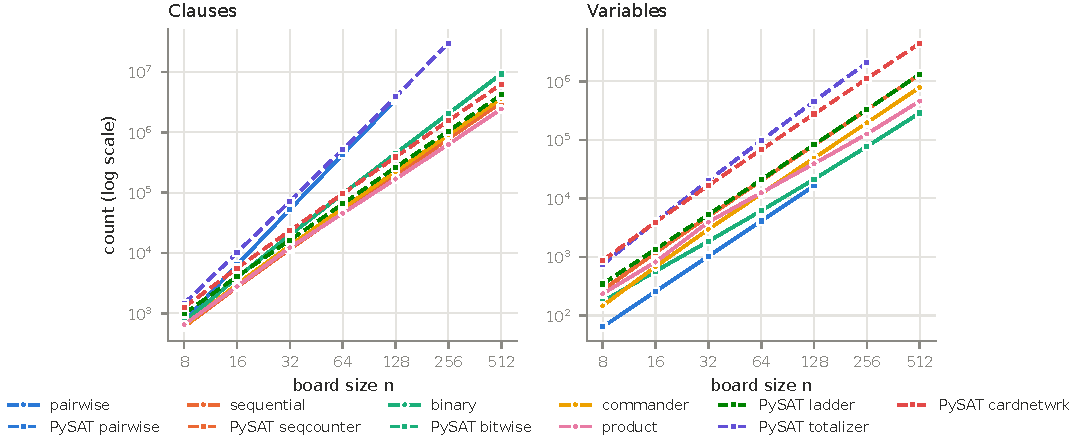
\includegraphics[width=\textwidth]{figures/fig_size.pdf}
\caption{Clauses and variables of $F_n(E)$ versus $n$ (log scales). Solid lines with circles: own encodings; dashed lines with squares: PySAT; one colour per encoding family.}\label{fig:size}
\end{figure}

\subsection{SAT solvers and encodings}\label{sec:sat}

Table~\ref{tab:sat-summary} and Figure~\ref{fig:sat} summarize the benchmark results across all eleven encodings and four SAT solvers. Of the 369 runs, 266 returned a valid solution, 88 proved unsatisfiability, 13 timed out, and 2 failed because the formula (PySAT totalizer, $n=512$) could not be built within 900\,s. Every returned solution passed the independent verification check. All 44 configurations proved $n=2$ and $n=3$ unsatisfiable in at most 7\,ms. Up to $n=64$, every configuration finished, mostly well under one second. Detailed per-run logs are stored in the CSV files of the repository.

\begin{table}[pos=!htb]
\caption{Largest board solved within 60\,s ($n_{\max}$, over $n\in\{8,16,32,\dots,512\}$) and solver time in seconds at $n=256$ ($t_{256}$). \TO: timeout; ``--'': not attempted; $^\dagger$: stopped by the memory cap (pairwise) or because the next formula could not be built within 900\,s (totalizer), not by a solver timeout.}\label{tab:sat-summary}
\centering\small
\begin{tabular}{@{}lrrrrrrrr@{}}
\toprule
Encoding & \multicolumn{2}{c}{CaDiCaL} & \multicolumn{2}{c}{Glucose} & \multicolumn{2}{c}{Kissat} & \multicolumn{2}{c}{MiniSat} \\
\cmidrule(lr){2-3}\cmidrule(lr){4-5}\cmidrule(lr){6-7}\cmidrule(lr){8-9}
 & $n_{\max}$ & $t_{256}$ & $n_{\max}$ & $t_{256}$ & $n_{\max}$ & $t_{256}$ & $n_{\max}$ & $t_{256}$ \\
\midrule
pairwise & 128$^\dagger$ & -- & 128$^\dagger$ & -- & 128$^\dagger$ & -- & 128$^\dagger$ & -- \\
PySAT pairwise & 128$^\dagger$ & -- & 128$^\dagger$ & -- & 128$^\dagger$ & -- & 128$^\dagger$ & -- \\
sequential & 256 & 33.3 & 64 & -- & 256 & 11.6 & 512 & 1.52 \\
PySAT seqcounter & 256 & 44.3 & 64 & -- & 512 & 9.65 & 512 & 1.44 \\
binary & 512 & 5.77 & 512 & 1.57 & 512 & 22.8 & 512 & 1.47 \\
PySAT bitwise & 256 & 6.90 & 512 & 1.95 & 512 & 14.9 & 512 & 1.36 \\
commander & 512 & 1.85 & 512 & 1.28 & 512 & 2.21 & 512 & 1.27 \\
product & 256 & 4.50 & 128 & TO & 512 & 3.29 & 512 & 0.77 \\
\midrule
PySAT ladder & 512 & 10.9 & 64 & -- & 512 & 6.74 & 512 & 2.16 \\
PySAT totalizer & 128 & TO & 256$^\dagger$ & 53.8 & 128 & TO & 256$^\dagger$ & 45.0 \\
PySAT cardnetwrk & 256 & 25.8 & 64 & -- & 512 & 13.1 & 512 & 2.21 \\
\bottomrule
\end{tabular}

\end{table}

\begin{figure}[pos=!htb]
\centering
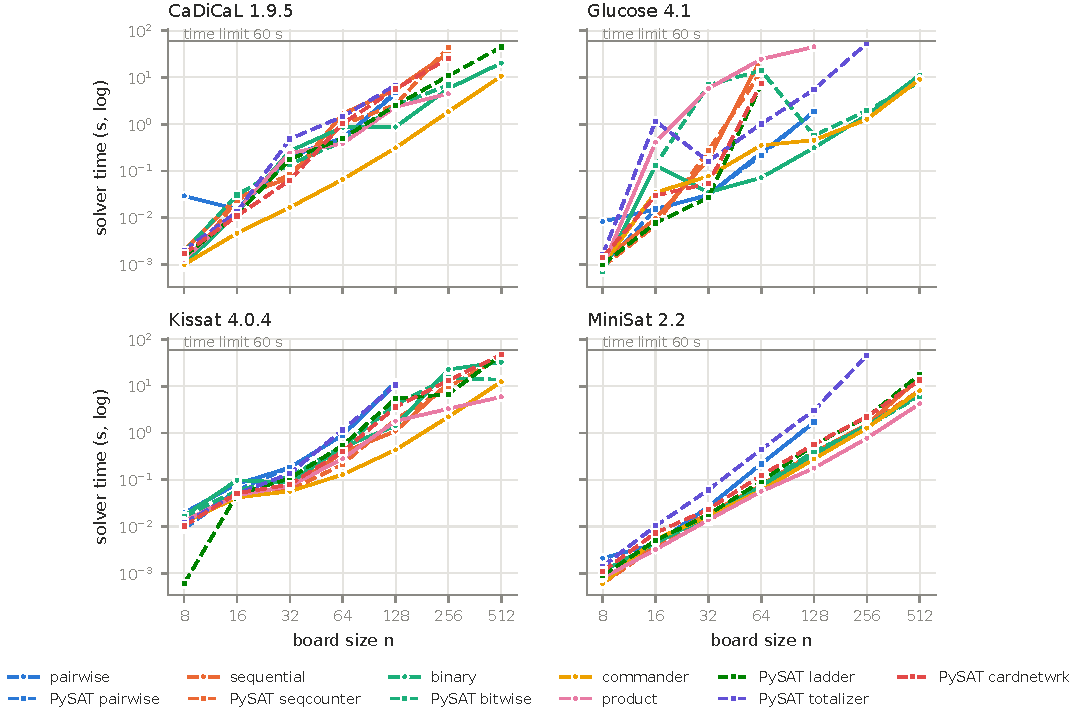
\includegraphics[width=\textwidth]{figures/fig_sat_time.pdf}
\caption{Solver time (log scale) versus board size for the eleven encodings with each SAT solver. A line ends at the last board solved within the 60\,s limit.}\label{fig:sat}
\end{figure}

\emph{(i) Cubic encodings do not scale.} The pairwise encodings were stopped at $n=128$ by the memory cap, and the PySAT totalizer timed out at $n=256$ with CaDiCaL and Kissat while its $n=512$ formula could not be built. Every other encoding solves $n=512$ with at least one solver.

\emph{(ii) Commander and binary are the most robust encodings.} They are the only encodings that solve $n=512$ with all four solvers. The commander encoding has the lowest time at $n=256$ with CaDiCaL (1.85\,s), Glucose (1.28\,s) and Kissat (2.21\,s). The product encoding gives the fastest configuration overall, with MiniSat (0.77\,s at $n=256$ and 4.22\,s at $n=512$), and is also fast with Kissat (5.91\,s at $n=512$), but it times out with Glucose at $n=256$ and with CaDiCaL at $n=512$.

\emph{(iii) The sequential counter suffers with the modern solvers.} Although it yields the second-smallest formula, its own and PySAT versions are the slowest subcubic encodings with CaDiCaL (33.3 and 44.3\,s at $n=256$, timeouts at $n=512$) and time out with Glucose from $n=128$, while MiniSat solves both at $n=512$ (14.9 and 8.2\,s). Formula size alone therefore does not predict solving time, in line with the observations of \citet{frisch2010sat}.

\emph{(iv) The solver matters as much as the encoding.} MiniSat~2.2, the oldest solver of the four, solves $n=512$ with every encoding whose formula could be built (eight configurations), Kissat with seven, and CaDiCaL and Glucose with three each. Glucose is also the least predictable: its time is not monotone in $n$ (PySAT bitwise needs 14.1\,s at $n=64$ but 0.57\,s at $n=128$). A plausible explanation is that CaDiCaL and Kissat spend effort on preprocessing and inprocessing, which pays off on hard industrial instances but is overhead on these large and structurally simple satisfiable formulas; we did not verify this hypothesis with solver statistics.

\emph{(v) Small formula differences can matter.} The own and PySAT versions of the binary encoding yield formulas of almost identical size (they differ by four clauses and four variables, Table~\ref{tab:size}), yet with CaDiCaL at $n=512$ ours finishes in 20.3\,s whereas PySAT bitwise times out. Such sensitivity is typical of CDCL search, so single-run differences of less than about a factor of two should not be over-interpreted.

\subsection{Effect of the redundant column constraints}\label{sec:ablation}

Table~\ref{tab:colalo} compares $F_n(E)$ with and without the redundant column ALO clauses, for four subcubic own encodings and the two most recent solvers. Over the 36 cases in which at least one of the two variants finished, the variant with the redundant clauses was faster in 28. In four cases (product with CaDiCaL at $n=128$, sequential with CaDiCaL at $n=256$, binary and product with Kissat at $n=512$) only the variant with the redundant clauses finished within the limit; the converse never occurred. The effect can exceed an order of magnitude: product with CaDiCaL needs 0.35\,s instead of 8.26\,s at $n=64$, and binary with CaDiCaL 5.55\,s instead of 55.2\,s at $n=256$. Although the column ALO clauses are logically implied, they cannot be obtained by unit propagation: deriving them requires a counting (pigeonhole) argument, which is notoriously hard for resolution-based solvers~\citep{haken1985intractability}. Stating them explicitly gives the solver this global information for free.

\begin{table}[pos=!htb]
\caption{Solver time (s) with and without the redundant column ALO clauses. \TO: timeout; ``--'': not attempted after a timeout at a smaller $n$.}\label{tab:colalo}
\centering\small
\begin{tabular}{@{}llrrrrrrrr@{}}
\toprule
Encoding & Solver & \multicolumn{2}{c}{$n=64$} & \multicolumn{2}{c}{$n=128$} & \multicolumn{2}{c}{$n=256$} & \multicolumn{2}{c}{$n=512$} \\
\cmidrule(lr){3-4}\cmidrule(lr){5-6}\cmidrule(lr){7-8}\cmidrule(lr){9-10}
 & & with & without & with & without & with & without & with & without \\
\midrule
sequential & CaDiCaL & 1.70 & 4.06 & 6.05 & 13.4 & 36.1 & TO & TO & -- \\
sequential & Kissat & 0.40 & 0.26 & 1.40 & 5.04 & 11.0 & 9.10 & TO & TO \\
commander & CaDiCaL & 0.07 & 0.09 & 0.34 & 0.58 & 1.97 & 4.01 & 10.6 & 16.9 \\
commander & Kissat & 0.13 & 0.17 & 0.50 & 0.75 & 2.06 & 1.81 & 12.8 & 23.6 \\
product & CaDiCaL & 0.35 & 8.26 & 2.35 & TO & 4.32 & -- & TO & -- \\
product & Kissat & 0.28 & 0.73 & 1.70 & 1.38 & 2.98 & 32.2 & 5.89 & TO \\
binary & CaDiCaL & 1.04 & 0.76 & 1.11 & 5.61 & 5.55 & 55.2 & 22.2 & 53.5 \\
binary & Kissat & 0.67 & 0.35 & 1.02 & 8.02 & 22.1 & 30.8 & 35.0 & TO \\
\bottomrule
\end{tabular}

\end{table}

\subsection{Comparison with CP and MIP solvers}

Table~\ref{tab:exact} and Figure~\ref{fig:exact} compare the two best SAT configurations of Section~\ref{sec:sat}, the product and commander encodings with MiniSat, with the other exact solvers. Every method proves $n=2$ and $n=3$ unsatisfiable within 7\,ms and returns a verified solution on every board it finishes.

\emph{MIP.} Within their licence limits, Gurobi and CPLEX solve every instance in at most 0.05\,s, as fast as SAT, presumably because on boards of this size their presolve and primal heuristics find a placement almost immediately, although the LP relaxation carries no information. Beyond $n=44$ (Gurobi) and $n=31$ (CPLEX) the free editions refuse the model. This is a limitation of the licences, not of the algorithms, so the results say nothing about how the MIP solvers would scale.

\emph{CP-SAT.} With the 0-1 model, CP-SAT solves $n=512$ in 10.2\,s and times out at $n=1000$. The integer model with three \textsc{AllDifferent} constraints is the most compact formulation ($n$ variables) but becomes the slowest beyond $n=128$ (53.0\,s at $n=256$, timeout at $n=512$). In a separate diagnostic run with logging enabled and a 5\,s limit, the presolve of CP-SAT expanded the $n=256$ integer model into 65\,536 new Boolean variables and stopped after presolve when the time budget was exhausted; with a single worker, this expansion dominates the run time.

\emph{SAT.} From $n=64$ on, the SAT configurations are the fastest. Product with MiniSat needs 0.77\,s at $n=256$ and 4.22\,s at $n=512$, i.e.\ 5.0 and 2.4 times less than CP-SAT with the 0-1 model, and it is the only approach that solves $n=1000$ (14.7\,s; commander with MiniSat needs 30.7\,s). The comparison remains favourable when model construction in Python is included: 5.65\,s against 12.6\,s at $n=512$, and 20.9\,s at $n=1000$ for a formula of 8.9 million clauses. Since CP-SAT is itself built on a CDCL engine with lazy clause generation, the gap is likely due to the formulation and to generic overheads (presolve, propagators for linear constraints, a single worker) rather than to a different search principle.

\begin{table}[pos=!htb]
\caption{Solver time (s) of the best SAT configurations and of the other exact methods. \TO: timeout after 60\,s; lic.: model rejected by the size-limited licence; ``--'': not attempted (beyond the licence limit or after a timeout). CPLEX CP Optimizer could not be run (Section~\ref{sec:experiments}).}\label{tab:exact}
\centering\small
\begin{tabular}{@{}rrrrrrr@{}}
\toprule
& \multicolumn{2}{c}{SAT (this work)} & \multicolumn{4}{c}{Other exact methods} \\
\cmidrule(lr){2-3}\cmidrule(lr){4-7}
$n$ & product+MiniSat & commander+MiniSat & CP-SAT int & CP-SAT 0-1 & Gurobi MIP & CPLEX MIP \\
\midrule
2 & $<$0.01 & $<$0.01 & $<$0.01 & $<$0.01 & $<$0.01 & $<$0.01 \\
3 & $<$0.01 & $<$0.01 & $<$0.01 & $<$0.01 & $<$0.01 & $<$0.01 \\
8 & $<$0.01 & $<$0.01 & $<$0.01 & $<$0.01 & $<$0.01 & $<$0.01 \\
16 & $<$0.01 & $<$0.01 & 0.02 & 0.01 & $<$0.01 & $<$0.01 \\
24 & $<$0.01 & $<$0.01 & 0.04 & 0.03 & $<$0.01 & 0.01 \\
31 & 0.01 & 0.01 & 0.06 & 0.04 & 0.02 & 0.01 \\
32 & 0.01 & 0.02 & 0.07 & 0.04 & 0.02 & lic. \\
40 & 0.06 & 0.03 & 0.11 & 0.07 & 0.03 & -- \\
44 & 0.04 & 0.03 & 0.14 & 0.09 & 0.05 & -- \\
64 & 0.06 & 0.06 & 0.33 & 0.22 & lic. & -- \\
128 & 0.18 & 0.28 & 2.03 & 1.63 & -- & -- \\
256 & 0.77 & 1.27 & 53.0 & 3.87 & -- & -- \\
512 & 4.22 & 8.02 & TO & 10.2 & -- & -- \\
1000 & 14.7 & 30.7 & -- & TO & -- & -- \\
\bottomrule
\end{tabular}

\end{table}

\begin{figure}[pos=!htb]
\centering
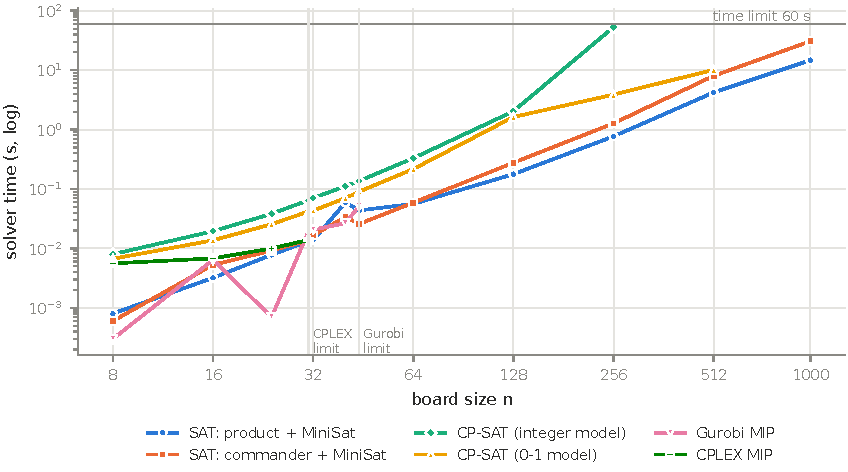
\includegraphics[width=\textwidth]{figures/fig_exact.pdf}
\caption{Solver time (log scale) of the best SAT configurations, CP-SAT (two models), Gurobi and CPLEX. Vertical lines mark the largest boards allowed by the CPLEX and Gurobi licences.}\label{fig:exact}
\end{figure}

\FloatBarrier
\section{Conclusion}\label{sec:conclusion}

In this assignment, we explored SAT-based approaches for solving the N-Queens problem by formulating cardinality constraints with eleven AMO encodings and evaluating them across four modern SAT solvers alongside exact CP and MIP baselines. The experimental results demonstrate the critical importance of choosing appropriate cardinality encodings for scalability, highlight the practical benefit of redundant propagation clauses, and illustrate the performance trade-offs between SAT, CP, and integer programming techniques.

In particular, the pairwise and PySAT totalizer encodings stop at $n=128$ and $n=256$, while the commander and binary encodings solve $n=512$ with all four solvers and the product encoding with MiniSat solves $n=1000$ in 14.7\,s. Keeping the redundant column ALO clauses made 28 of 36 compared runs faster. CP-SAT reached $n=512$ with the 0-1 model, and Gurobi and CPLEX were as fast as SAT within their licence limits ($n\le44$ and $n\le31$).

\section*{Declaration of generative AI and AI-assisted technologies}
During the preparation of this assignment, the author utilized AI-assisted tools including ChatGPT, Gemini Antigravity, GitHub Copilot, etc., for code debugging, structuring benchmark scripts, grammar checking, and LaTeX formatting. The author reviewed and verified all experimental code, results, and writings.

\section*{Data availability}\label{sec:data}
The source code, the raw CSV results, the logs and the scripts that generate every table and figure of this report are available at \url{https://github.com/phuck40clnq/INT3011}.

\bibliographystyle{cas-model2-names}
\bibliography{refs}

\end{document}
